\documentclass[]{paper}
\usepackage{amsmath}
\usepackage{amssymb}
\usepackage{float}
\usepackage{tikz}
\usetikzlibrary{positioning,arrows.meta,fit,shapes.geometric}

\newcommand{\keep}{\textsc{keep}}
\newcommand{\edit}{\textsc{edit}}
\newcommand{\drop}{\textsc{drop}}
\newcommand{\run}[1]{\texttt{#1}}

\begin{document}

\title{The DiffusEdit Method}

\author[*]{Tatva Agarwal}
\author[*]{Vedant Kulkarni}
\author[*]{Bysani Vedavyas}
\author[*]{Venya Velmurugan}

\affiliation[]{IIIT Hyderabad}

\contribution[*]{Equal contribution; authors listed alphabetically.}

\abstract{
DiffusEdit updates an outdated Wikipedia article from a few evidence passages. Small heads on the hidden states of a frozen diffusion language model choose which sentences to change and which of their tokens are stale, the model infills the stale tokens, and a ranking picks one of the infilled sentences. This document explains each part of the current method with one worked example, treats every earlier run and every ablation as a variation of that method, and reports the results of every variation in tables and plots. With the learned ranking the repair gains 0.054 ROUGE-L over leaving the sentence unchanged on the synthetic test set, and a fine-tuned T5 editor gains 0.099 on the same sentences.
}

\date{}
\correspondence{\email{vedant.kulkarni@students.iiit.ac.in}}

\maketitle{}

\section{Introduction}
\label{sec:intro}

An article is a list of sentences, and an update replaces some of them. The input is the outdated article and a few evidence passages that state the new facts. The output is the updated article. Each source sentence has one of three labels. A \keep{} sentence is still correct, an \edit{} sentence needs a change, and a \drop{} sentence should be removed.

One test article is the example throughout. Its first sentence reads \emph{Drumry railway station serves the Drumry and Linnvale area of Clydebank, West Dunbartonshire, Scotland}, and one evidence passage reads \emph{Drumry station serves homes in Drumry and Linnvale, districts of Leigh in West Dunbartonshire}. The gold update replaces \emph{Clydebank} with \emph{Leigh} and changes nothing else. The second sentence of the article, about the operator of the station, is a \keep{} sentence.

DiffusEdit repairs an \edit{} sentence in place. It masks the stale tokens, fills the masks with a frozen masked diffusion model, and keeps one of the filled sentences. The method is built on LLaDA-8B-Base \citep{nie-etal-2025-llada}, a masked diffusion language model that predicts masked tokens from both sides of the context. \Cref{sec:method} defines each part of the current method on the example. \Cref{sec:data,sec:protocol,sec:metrics} give the data, the protocol and the metrics. \Cref{sec:experiments} lists every run as a variation of the current method, and \cref{sec:results} reports them.

\section{Method}
\label{sec:method}

\Cref{fig:pipeline} shows one round. One forward pass over the evidence followed by the article gives a hidden state for every token. Small trained heads on these states make every decision except the infilling, and LLaDA itself is never trained.

\begin{figure}[t]
\centering
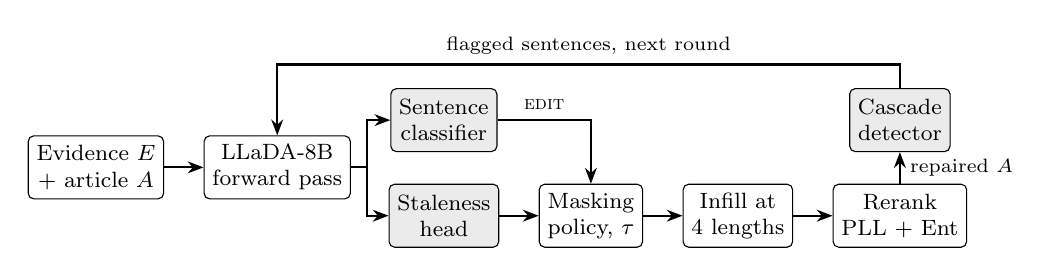
\begin{tikzpicture}[
  node distance=4mm and 5mm,
  box/.style={draw, rounded corners=2pt, align=center, font=\footnotesize, minimum height=8mm, inner sep=3pt},
  head/.style={box, fill=black!8},
  arr/.style={-{Stealth[length=2mm]}, thick}]
\node[box] (in) {Evidence $E$\\ + article $A$};
\node[box, right=of in] (llada) {LLaDA-8B\\ forward pass};
\node[head, right=of llada, yshift=6mm] (cls) {Sentence\\ classifier};
\node[head, below=of cls] (stale) {Staleness\\ head};
\node[box, right=of stale] (mask) {Masking\\ policy, $\tau$};
\node[box, right=of mask] (fill) {Infill at\\ 4 lengths};
\node[box, right=of fill] (rank) {Rerank\\ PLL + Ent};
\node[head, above=of rank] (casc) {Cascade\\ detector};
\draw[arr] (in) -- (llada);
\draw[arr] (llada.east) -- ++(2mm,0) |- (cls.west);
\draw[arr] (llada.east) -- ++(2mm,0) |- (stale.west);
\draw[arr] (cls.east) -| node[pos=0.25, above, font=\scriptsize] {\edit{}} (mask.north);
\draw[arr] (stale) -- (mask);
\draw[arr] (mask) -- (fill);
\draw[arr] (fill) -- (rank);
\draw[arr] (rank) -- node[right, font=\scriptsize] {repaired $A$} (casc);
\draw[arr] (casc.north) -- ++(0,3mm) -| node[pos=0.25, above, font=\scriptsize] {flagged sentences, next round} (llada.north);
\end{tikzpicture}

\caption{One round of DiffusEdit. Grey boxes are trained heads on the frozen LLaDA states. The cascade detector runs after the round and selects the sentences of the next round.}
\label{fig:pipeline}
\end{figure}

\subsection{Forward Pass}

The input sequence is the evidence passages followed by the article. LLaDA is run once over this sequence without any mask, and the hidden state of every token at every block is kept. A hidden state is the vector that the model computes for one token at one block, 4,096 numbers for LLaDA-8B\@. The heads read the states of the article tokens, and the attention head also reads the states of the evidence tokens. For the example, the sequence holds the two evidence passages and then the two sentences of the article, and the pass runs once per round.

\subsection{Sentence Classifier}

The sentence classifier assigns \keep{}, \edit{} or \drop{} to each article sentence. It is a linear layer on the mean hidden state of the sentence's tokens at block 24 of the 32 blocks. Block 24 is used because its val macro-F1 is higher than that of block 32. The classifier is trained with cross-entropy on the train split and the label with the highest probability is taken. For the example it labels the first sentence \edit{} and the second \keep{}.

\subsection{Staleness Head}

The staleness head scores each token of an \edit{} sentence with the probability that it is stale. The head compares the token's state with the states of the evidence tokens through a learned attention with one extra null slot, so that a token can attend to nothing when the evidence does not mention it. The attention output and the token state go through a small feed-forward layer to one score. The head is trained with binary cross-entropy on the derived stale tokens of the train split, which are the tokens that the word-level difference between the source and the gold sentence marks as changed.

\subsection{Masking Policy}

The masking policy turns token scores into spans of masks. Tokens with a score of at least $\tau = 0.85$ are masked. An empty mask falls back to the top fifth of the sentence, a mask over half of the sentence keeps its top half, and each span is widened to whole words. A token can be masked at most three times over all rounds. For the example the head masks two spans, \emph{Clydebank} and \emph{Scotland}. The first span is stale and the second is not.

\subsection{Candidates}

Each span of $n$ masks is infilled at four lengths, $0$, $\lceil n/2 \rceil$, $n$ and $n+2$, so that the repair can delete, shorten, keep or lengthen the span. LLaDA fills the masks greedily in 8 steps, with the whole evidence and article as context. Each filled sentence is a \emph{candidate}, and the set of candidates for one sentence is its \emph{pool}. Spans are decided left to right. For span $i$ each candidate is sampled together with the later spans masked at their own length, so every candidate is a whole sentence. The winner of span $i$ is committed and span $i+1$ is decided next.

Four more candidates per span copy an evidence phrase into the span verbatim. The phrases are the named entities of the evidence that the sentence lacks, of the masked text's entity type, and the four kept are those whose tokens have the highest mean log-probability under LLaDA in the span. A sampled fill can only hold words with a high probability under the model, while these candidates hold the evidence's words whatever their probability.

\subsection{Candidate Rules}

Four rules were added after the first test run, in response to failures read in the val outputs (\cref{sec:protocol}).
\begin{itemize}
\item An \emph{edit penalty} subtracts 0.1 times the word edit distance between the candidate and the sentence before repair, so that a candidate is charged for every changed word \citep{chen-etal-2022-converge}.
\item The \emph{rejection rule} subtracts 100 from a candidate that adds a capitalised word or a number found in neither the evidence nor the sentence before repair. A rejected candidate still wins when every candidate is rejected.
\item The \emph{evidence veto} unmasks a span whose words all occur somewhere in the evidence, because such a span is not contradicted by the evidence.
\item The \emph{span cap} leaves a sentence unrepaired when its mask has more than two spans, because such masks were mostly wrong.
\end{itemize}

\subsection{Ranking}

The \emph{heuristic ranking} scores each candidate by $0.5\,\mathrm{PLL} + 0.5\,\mathrm{Ent}$, less the penalty and the rejection. PLL is the pseudo-log-likelihood of the sentence under LLaDA, the mean log-probability of each token when it alone is masked. Ent is the probability that the VitaminC verifier \citep{schuster-etal-2021-vitaminc} assigns to the best evidence passage supporting the sentence. A deletion candidate wins only when its score is at least 0.1 above the best rewrite, because removing a span also removes the claim the verifier would have checked.

\Cref{tab:example} shows the pool of the example's first span under this ranking. The three sampled fills add a place name that the evidence does not hold, so the rejection rule removes them, and the deletion wins. No candidate holds \emph{Leigh}, so the best candidate of the pool scores below the gold update. Under the sentence metric the deletion still scores above the unchanged sentence, because the stale word is gone.

\begin{table}[H]
\caption{The pool of the example's first span, \emph{Clydebank}. Score is the heuristic score. ROUGE-L is against the gold update. The second span, \emph{Scotland}, is decided afterwards and is kept.}
\label{tab:example}
\centering
\footnotesize
\begin{tabular}{llccrc}
\toprule
Length & Fill & PLL & Ent & Score & ROUGE-L \\
\midrule
0 & (deleted) & $-0.32$ & 0.002 & $-0.26$ & 0.963 \\
2 & Barrhead & $-0.15$ & 0.002 & $-100.18$ & 0.929 \\
3 & Sighthill & $-0.14$ & 0.002 & $-100.17$ & 0.929 \\
5 & the northern suburbs of Glasgow & $-0.22$ & 0.002 & $-100.61$ & 0.813 \\
\bottomrule
\end{tabular}
\end{table}

The \emph{learned ranking} replaces the score with a classifier. Every candidate is a whole sentence, so the logged pools of a run can be ranked again without a model pass. Each candidate gets features from its logged scores and from its text. The score features are PLL, Ent, their differences from the best of the pool, and their ranks. The length features are the ratio of the fill length to the span length and the length rule the fill came from. The text features are the word edit distance to the source, the ROUGE-L against the source, the counts of capitalised words and numbers the candidate adds, split by whether the evidence holds them, the count of such words it drops, and the mean and minimum confidence of the sampler. The unchanged source joins every pool as one more candidate, so the ranking can leave a sentence as it is. A gradient-boosted tree classifier is fit on the pools of the val articles to predict whether a candidate has the best ROUGE-L of its pool, and the candidate with the highest predicted probability is the output.

\Cref{tab:learned} shows a pool where the two rankings differ. The sampled fill at the same length reproduces the source word, its PLL is the highest of the pool, and the edit penalty charges the evidence copy for its one changed word, so the heuristic leaves the sentence unchanged. The learned ranking prefers the evidence copy, which equals the gold update.

\begin{table}[H]
\caption{A test pool where the rankings differ. The source is \emph{Prior to European contact, the Batswana lived as herders and farmers under tribal rule}, the span is \emph{European}, and the gold update replaces it with \emph{Roman}. Score is the heuristic score, and ROUGE-L is against the gold update.}
\label{tab:learned}
\centering
\footnotesize
\begin{tabular}{llccrc}
\toprule
Kind & Fill & PLL & Ent & Score & ROUGE-L \\
\midrule
deletion & (deleted) & $-0.86$ & 0.021 & $-0.52$ & 0.963 \\
sampled, same length & European & $-0.56$ & 0.021 & $-0.27$ & 0.929 \\
sampled, longer & European and missionary & $-0.65$ & 0.061 & $-0.49$ & 0.867 \\
evidence copy & Roman & $-0.74$ & 0.041 & $-0.45$ & 1.000 \\
\bottomrule
\end{tabular}
\end{table}

\subsection{Rounds and Cascades}

A repair can make another sentence stale. If a birth date changes, a sentence that states an age is now wrong, although nothing in the evidence mentions it. Such a sentence is a \emph{cascade} sentence. After a round, a cascade detector flags sentences outside the repaired set, and the next round repairs them. The loop runs at most three rounds.

Three detectors were built. The \emph{consequence head} scores a pair of a repaired sentence and another sentence from their states before and after the repair, and flags the pair when the score is above $\tau_c = 0.35$. \emph{Staleness delta} flags a sentence whose staleness scores rise after the round. \emph{Edited as evidence} appends the repaired sentences to the evidence, so that the next pass covers them, and flags the sentences the classifier then labels \edit{}. A loop with no detector stops after one round.

\section{Data}
\label{sec:data}

The synthetic set is built from Wikipedia articles. One to three named entities of an \edit{} sentence are swapped for entities of the same spaCy type, and language model agents write evidence passages for the change. The set is used in reversed form. The real Wikipedia sentence is the outdated source, the swapped sentence is the gold update, and the evidence states the swapped values. In the forward direction a repair restored the real values without the evidence, because they occur in LLaDA's pretraining text. In the example, \emph{Clydebank} is the real value and \emph{Leigh} the swapped one.

\begin{table}[H]
\caption{Splits of the reversed synthetic set. Supported articles have at least one \edit{} sentence whose new words all occur in the evidence or the source sentence. Linked articles hold a cascade sentence labelled by hand.}
\label{tab:data}
\centering
\footnotesize
\begin{tabular}{lrrr}
\toprule
 & Train & Val & Test \\
\midrule
Articles & 12,180 & 1,564 & 1,602 \\
\keep{} / \edit{} / \drop{} sentences & 27,061 / 12,360 / 3,062 & 3,472 / 1,575 / 414 & 3,500 / 1,684 / 428 \\
Evidence passages per article & 2.14 & 2.16 & 2.15 \\
Supported articles (\edit{} sentences) & & & 901 (1,670) \\
Linked articles (cascade sentences) & & & 220 (232) \\
\bottomrule
\end{tabular}
\end{table}

The generator guarantees that every new value of an \edit{} sentence occurs verbatim in the evidence and that no old value occurs anywhere in it. The rejection rule, the evidence veto and the evidence-copy candidates rely on these two guarantees. Update data taken from Wikipedia revisions, such as FRUIT \citep{iv-etal-2022-fruit}, guarantees neither.

\section{Protocol}
\label{sec:protocol}

Heads are fit on the train split. The val split sets early stopping, every threshold and every repair setting. The test split is scored once per configuration. FRUIT val and test are not used, and FRUIT train is used for one stress set only.

\Cref{fig:order} shows the order of the runs. The first single-round runs on test used the base setting without the candidate rules. The run with attention-head masks, \run{fix-attention}, gained 0.009 ROUGE-L over copy and failed a gate of 0.01. Its val outputs were then read. The ranking preferred the longest candidate for 44\% of the spans, masks covered names and dates that were not stale, and for 15\% of the sentences the gold update could not be produced from the input. The four candidate rules and the evidence-copy candidates were added in response. The base setting, v1 with the four rules, and v2 with the rules and the evidence copies were compared on 200 val articles that had not been read, and v2 was chosen. Its test run is \run{fix-tuned}. The learned ranking was then fit on the v2 pools of the same 200 val articles and applied once to the test pools of \run{fix-tuned}, which gives \run{fix-rerank}.

\begin{figure}[t]
\centering
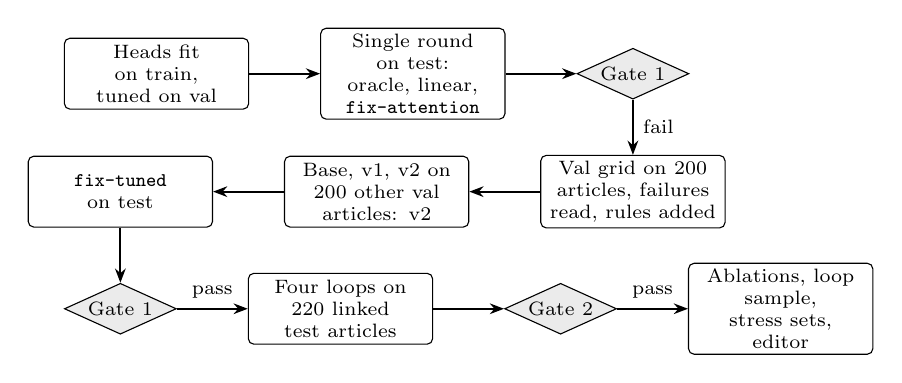
\begin{tikzpicture}[
  node distance=5mm and 9mm,
  box/.style={draw, rounded corners=2pt, align=center, font=\scriptsize, minimum height=9mm, text width=22mm, inner sep=2pt},
  gate/.style={draw, diamond, aspect=2.2, align=center, font=\scriptsize, inner sep=1pt, fill=black!8},
  arr/.style={-{Stealth[length=1.8mm]}, thick}]
\node[box] (heads) {Heads fit on train,\\ tuned on val};
\node[box, right=of heads] (fix) {Single round on test:\\ oracle, linear,\\ \run{fix-attention}};
\node[gate, right=of fix] (g1) {Gate 1};
\node[box, below=7mm of g1] (grid) {Val grid on 200\\ articles, failures\\ read, rules added};
\node[box, left=of grid] (fresh) {Base, v1, v2 on\\ 200 other val\\ articles: v2};
\node[box, left=of fresh] (tuned) {\run{fix-tuned}\\ on test};
\node[gate, below=7mm of tuned] (g1b) {Gate 1};
\node[box, right=of g1b] (loops) {Four loops on\\ 220 linked\\ test articles};
\node[gate, right=of loops] (g2) {Gate 2};
\node[box, right=of g2] (rest) {Ablations, loop\\ sample, stress sets,\\ editor};
\draw[arr] (heads) -- (fix);
\draw[arr] (fix) -- (g1);
\draw[arr] (g1) -- node[right, font=\scriptsize] {fail} (grid);
\draw[arr] (grid) -- (fresh);
\draw[arr] (fresh) -- (tuned);
\draw[arr] (tuned) -- (g1b);
\draw[arr] (g1b) -- node[above, font=\scriptsize] {pass} (loops);
\draw[arr] (loops) -- (g2);
\draw[arr] (g2) -- node[above, font=\scriptsize] {pass} (rest);
\end{tikzpicture}

\caption{Order of the runs. A failed gate stops every later stage. Gate 1 failed once, and the repair setting was then chosen again on val.}
\label{fig:order}
\end{figure}

The full test set does not fit the GPU budget for every ablation. The ablation sample holds 300 of the 901 supported test articles, with 557 \edit{} sentences, and the loop sample 300 of the 1,602 test articles. Both were drawn with seed 42, and each comparison on a sample is made against the reference run restricted to the same articles.

Three stress sets break the guarantees of the generator on the 200 val articles that chose v2. In the \emph{missing-value} set, for 183 of the 367 \edit{} sentences, every passage that holds a new value of the sentence is removed. In the \emph{old-value} set, one passage per \edit{} sentence is added that mentions the old values in another context and none of the new values. The \emph{FRUIT} set holds 200 FRUIT train articles with a stale \edit{} sentence.

Every interval is a 95\% bootstrap interval that resamples whole articles, and every comparison between runs is paired over articles. Decoding is greedy, so a repair run gives the same output for the same head. The staleness head of every repair run was trained with seed 42, so the intervals cover the sampling of articles and not the training seed.

\section{Metrics}
\label{sec:metrics}

Every sentence metric is computed over all gold \edit{} sentences of the articles a run reads, and a sentence the run leaves unchanged is scored as its source. \emph{ROUGE-L} is the ROUGE-L F1 of the output sentence against the gold update. \emph{Copy} is the same score for the unchanged source, and the \emph{gain} of a run is its ROUGE-L minus copy. Copy scores 0.875 on test, because an \edit{} sentence changes a few words and keeps the rest, so a gain of 0.04 is a third of what copy leaves. \emph{Pool} is the best ROUGE-L over every candidate the run generated, and the difference between pool and ROUGE-L is the loss due to the ranking.

Three value-level scores look only at the swapped values. \emph{Exact match} is the share of output sentences equal to the gold update, ignoring case and spacing. \emph{New-value recall} is the share of gold new values that occur in the output as whole words. \emph{Old value kept} is the share of old values still in the output, and lower is better.

The article metrics compare the output article with the gold article. \emph{UpdateROUGE-L} \citep{iv-etal-2022-fruit} is ROUGE-L between the output sentences that differ from the source and the gold sentences that differ from the source. An unchanged output sentence adds nothing to the output side, so a system that changes more sentences scores higher. \emph{Cascade ROUGE-L} is the same score restricted to the cascade sentences, \emph{cascade recall} is the share of cascade sentences a detector flags, and \emph{\keep{} verbatim} is the share of gold \keep{} sentences left unchanged.

The sentence classifier is scored by macro-F1 over the three labels, and the staleness heads by the area under the precision-recall curve (PR-AUC) over the tokens of \edit{} sentences, of which 11.3\% are stale.

\section{Experiments}
\label{sec:experiments}

Every run is a variation of the current method along one axis. \Cref{tab:runs} lists them. The masks axis replaces the attention head's masks with the derived stale tokens (oracle masks) or with the masks of a linear head on the token state alone. The evidence axis removes the evidence from the input. The setting axis compares the base setting, v1 and v2. The rules axis removes one candidate rule at a time from v2. The candidates axis restricts the lengths to $n$ only, and the score axis ranks by PLL only or by the verifier only. The ranking axis compares the heuristic and the learned ranking on the same pools. The detector axis changes the cascade detector of the loop, and the labels axis replaces the predicted sentence labels with the gold labels. The data axis runs the base setting and v2 on the stress sets. The editor baseline is flan-t5-large fine-tuned on the train split to write the updated article from the outdated article and the evidence, in the style of EDIT5 \citep{iv-etal-2022-fruit}.

\begin{table}[H]
\caption{Every run as a variation of the current method. The current method is attention-head masks, the v2 setting, the learned ranking and the consequence loop. Sentence counts are gold \edit{} sentences.}
\label{tab:runs}
\centering
\footnotesize
\setlength{\tabcolsep}{4pt}
\begin{tabular}{llllr}
\toprule
Axis & Run & Change from the current method & Set & Sentences \\
\midrule
Masks & \run{fix-oracle} & oracle masks, base setting & test & 1,670 \\
 & \run{fix-predicted} & linear-head masks, base setting & test & 1,670 \\
 & \run{fix-attention} & base setting & test & 1,670 \\
 & \run{fix-oracle-tuned} & oracle masks & sample & 557 \\
Evidence & \run{fix-oracle-noev} & oracle masks, base setting, no evidence & test & 1,670 \\
Setting & \run{repair-val2-base}, \run{-v1}, \run{-v2} & base, v1, v2 & val & 367 \\
 & \run{fix-tuned} & heuristic ranking & test & 1,670 \\
Rules & \run{abl-no-penalty} & v2 without the edit penalty & sample & 557 \\
 & \run{abl-no-reject} & v2 without the rejection rule & sample & 557 \\
 & \run{abl-no-veto} & v2 without the evidence veto & sample & 557 \\
 & \run{abl-no-cap} & v2 without the span cap & sample & 557 \\
 & \run{abl-no-copy} & v2 without the evidence-copy candidates & sample & 557 \\
Candidates & \run{abl-same} & oracle masks, base, length $n$ only & sample & 557 \\
Score & \run{abl-pll} & oracle masks, base, PLL only & sample & 557 \\
 & \run{abl-verifier} & oracle masks, base, verifier only & sample & 557 \\
Ranking & \run{fix-rerank} & none & test & 1,670 \\
 & \run{fix-oracle-rerank} & oracle masks & sample & 557 \\
Detector & \run{loop-none} & one round, no detector & linked & 220 articles \\
 & \run{loop-staleness\_delta} & staleness delta & linked & 220 articles \\
 & \run{loop-edited\_as\_evidence} & edited as evidence & linked & 220 articles \\
 & \run{loop-consequence} & heuristic ranking & linked & 220 articles \\
Labels & \run{loop-oracle-labels} & gold sentence labels & linked & 220 articles \\
Data & \run{stress-missing-*} & base and v2 on the missing-value set & val & 367 \\
 & \run{stress-oldvalue-*} & base and v2 on the old-value set & val & 367 \\
 & \run{stress-fruit-*} & base and v2 on FRUIT train & FRUIT & 408 \\
Baseline & \run{editor} & fine-tuned T5 editor & test & 1,670 \\
\bottomrule
\end{tabular}
\end{table}

\section{Results}
\label{sec:results}

\subsection{Heads}

\Cref{fig:heads} shows the heads with and without evidence. The sentence classifier reaches macro-F1 0.823 over five seeds, with a spread of 0.002. Without the evidence in the input it falls to 0.332, which is the score of a constant prediction, so the label comes from the comparison between the sentence and the evidence and not from the sentence alone. A MiniLM baseline on the same task reaches 0.487. The attention staleness head reaches PR-AUC 0.831 against 0.739 for the linear head, and it falls to 0.625 with the evidence of another article and to 0.718 with no evidence, so its score depends on the evidence. The consequence head reaches AUROC 0.931 on 1,106 sentence pairs.

\begin{figure}[H]
\centering
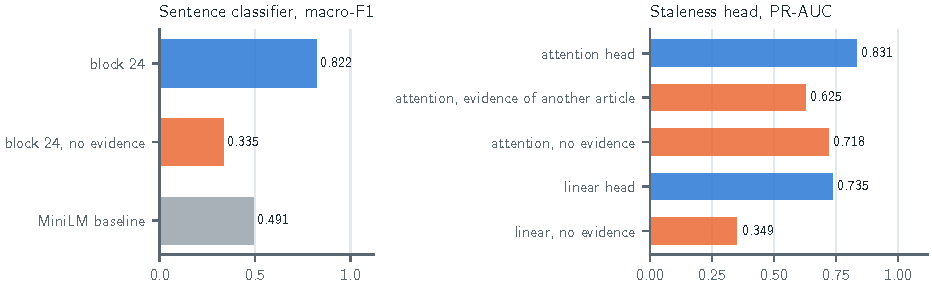
\includegraphics[width=\linewidth]{figures/heads.pdf}
\caption{Test scores of the heads trained with seed 42. Orange bars are controls without the evidence or with the evidence of another article.}
\label{fig:heads}
\end{figure}

\subsection{Masks}

\Cref{fig:ladder} shows, for each single-round run, where the chosen candidate sits between copy and the best candidate of the pool. Oracle masks with the base setting gain 0.037, and the same masks without evidence lose 0.021, so the gain comes from the evidence. The linear head's masks gain nothing, and the attention head's masks gain 0.009 with the base setting. With the v2 setting the same masks gain 0.038, and oracle masks with v2 gain 0.064 on the sample. The pool of every run with the v2 setting reaches about 0.95 with the attention head and 0.98 with oracle masks, so the masks set the ceiling and the ranking sets how much of the ceiling is reached.

\begin{figure}[H]
\centering
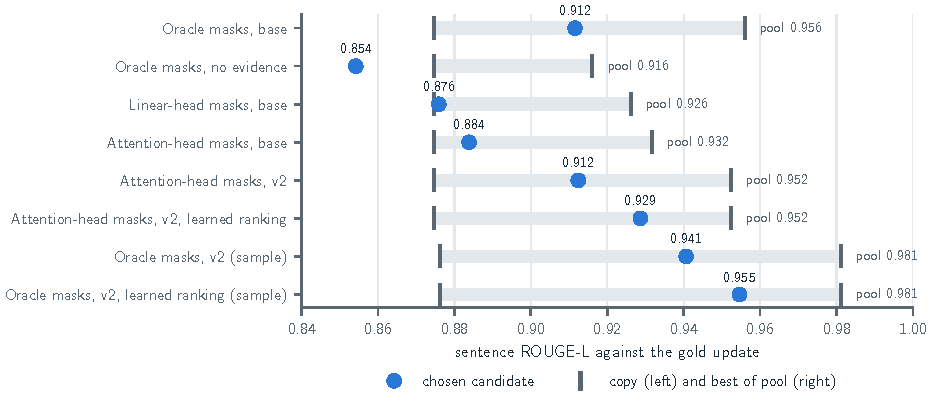
\includegraphics[width=\linewidth]{figures/ladder.pdf}
\caption{Sentence ROUGE-L of each single-round run. The grey bar runs from copy to the best candidate of the pool, and the dot is the chosen candidate. Test runs cover 1,670 sentences and sample runs 557.}
\label{fig:ladder}
\end{figure}

\Cref{fig:gains} gives the same runs as gains over copy with their intervals, together with the editor.

\begin{figure}[H]
\centering
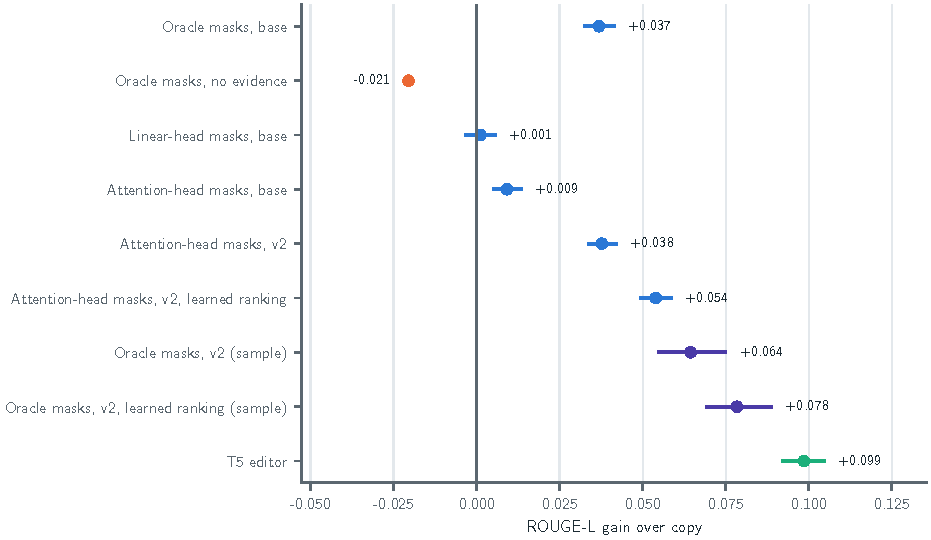
\includegraphics[width=\linewidth]{figures/gains.pdf}
\caption{Sentence ROUGE-L gain over copy with 95\% article bootstrap intervals.}
\label{fig:gains}
\end{figure}

\subsection{Repair Rules}

\Cref{fig:rules} shows each rule removed from v2 on the ablation sample. Removing the edit penalty, the rejection rule or the evidence veto lowers ROUGE-L by an amount whose interval excludes zero. Removing the span cap or the evidence-copy candidates changes ROUGE-L by less than the interval width. The learned ranking on the same pools raises ROUGE-L by more than any rule.

\begin{figure}[H]
\centering
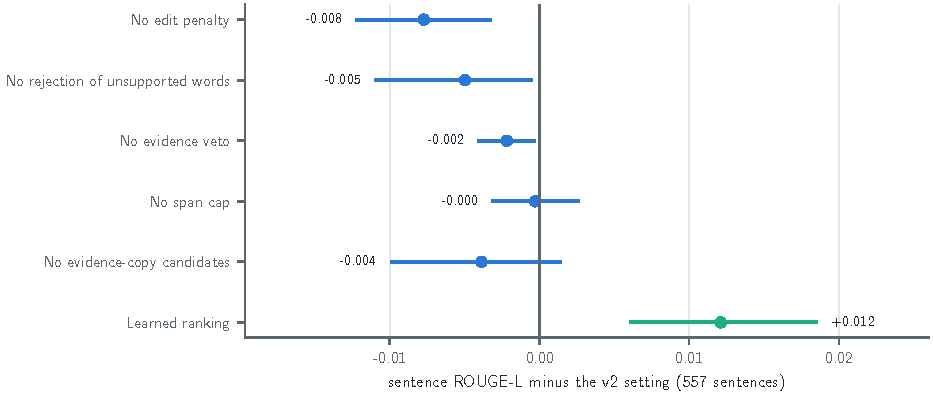
\includegraphics[width=\linewidth]{figures/rules.pdf}
\caption{Each repair rule removed from the v2 setting, and the learned ranking added to it, as the sentence ROUGE-L difference from \run{fix-tuned} on the 557 sentences of the ablation sample.}
\label{fig:rules}
\end{figure}

\subsection{Candidate Lengths and Scores}

\Cref{fig:lengths} shows the candidate and score variations with oracle masks and the base setting. Same-length candidates score 0.008 above the four-length set, because with the base setting the ranking preferred the longest candidate for 44\% of the spans, and the longer candidates were mostly wrong. The edit penalty of v2 removes this preference. Ranking by PLL alone is within noise of the combined score, and ranking by the verifier alone is 0.006 lower, so the verifier adds little on its own.

\begin{figure}[H]
\centering
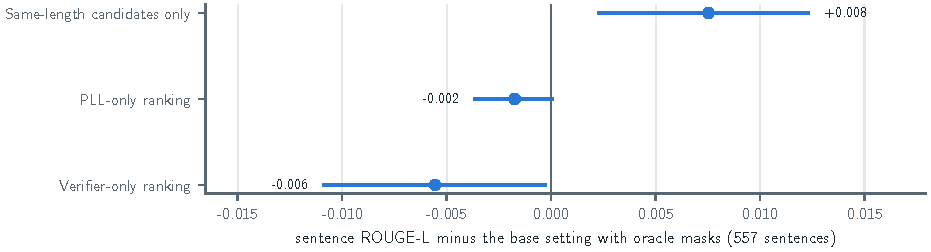
\includegraphics[width=\linewidth]{figures/lengths.pdf}
\caption{Candidate lengths and scores with oracle masks and the base setting, as the sentence ROUGE-L difference from \run{fix-oracle} on the 557 sentences of the ablation sample.}
\label{fig:lengths}
\end{figure}

\subsection{Ranking}

\Cref{tab:ranking} and \cref{fig:values} compare the two rankings on the 1,670 test sentences. The learned ranking raises ROUGE-L from 0.912 to 0.929, which is a paired difference of 0.016 $[0.013, 0.020]$, and it raises exact match from 0.253 to 0.323 and new-value recall from 0.395 to 0.499. It also lowers the share of old values kept from 0.495 to 0.261. Under five-fold cross-validation over the val articles the gain was 0.019, and three tree sizes, a logistic regression and extra training pools from the other val runs all gave gains between 0.012 and 0.020. On the oracle-mask sample the learned ranking raises ROUGE-L from 0.941 to 0.955.

\begin{table}[H]
\caption{The two rankings and the editor on the 1,670 \edit{} sentences of the supported test articles, with 95\% article bootstrap intervals. Lower is better for old value kept.}
\label{tab:ranking}
\centering
\footnotesize
\begin{tabular}{lcccc}
\toprule
System & ROUGE-L & Exact match & New-value recall & Old value kept \\
\midrule
Copy & 0.875 & 0.000 & 0.031 & 1.000 \\
Heuristic ranking (\run{fix-tuned}) & 0.912 & 0.253 $[0.232, 0.274]$ & 0.395 $[0.373, 0.417]$ & 0.495 $[0.470, 0.521]$ \\
Learned ranking (\run{fix-rerank}) & 0.929 & 0.323 $[0.301, 0.345]$ & 0.499 $[0.476, 0.521]$ & 0.261 $[0.240, 0.281]$ \\
T5 editor & \textbf{0.973} & \textbf{0.767} $[0.747, 0.787]$ & \textbf{0.887} $[0.873, 0.902]$ & \textbf{0.100} $[0.086, 0.115]$ \\
\bottomrule
\end{tabular}
\end{table}

\begin{figure}[H]
\centering
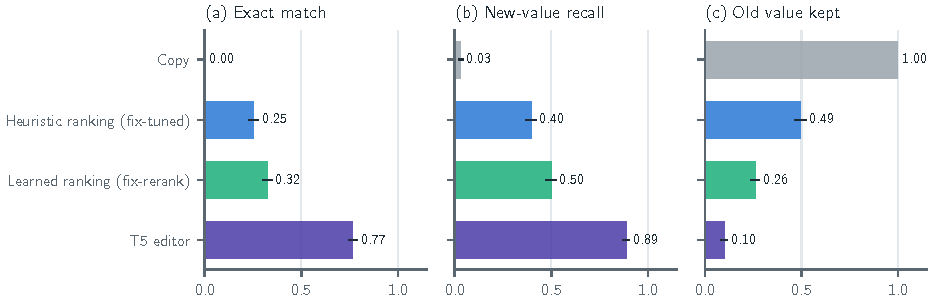
\includegraphics[width=\linewidth]{figures/values.pdf}
\caption{Value-level scores on the 1,670 test sentences, with 95\% article bootstrap intervals.}
\label{fig:values}
\end{figure}

\Cref{fig:picks} shows what kind of candidate each ranking chooses. The heuristic ranking leaves 703 of the 1,670 sentences equal to the source, including the 209 that the span cap leaves unrepaired, and chooses an evidence-copy candidate for 286. The learned ranking leaves 279 unchanged and chooses an evidence copy for 519 and a deletion for 283. A deletion removes the stale value and scores above a wrong replacement under ROUGE-L, and the deletion choices carry 21\% of the test gain. A variant that never chooses a deletion gains 0.017 in the same cross-validation, with a higher exact match, and has not been scored on test.

\begin{figure}[H]
\centering
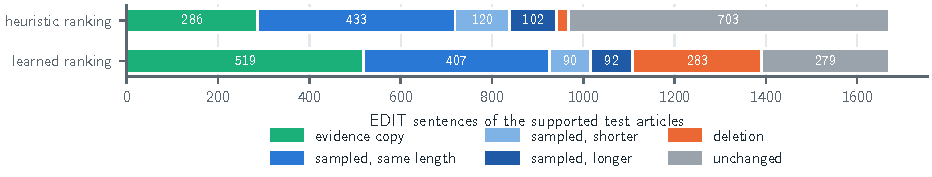
\includegraphics[width=\linewidth]{figures/picks.pdf}
\caption{The kind of candidate each ranking chooses on the 1,670 test sentences. Unchanged covers the 209 sentences the span cap leaves unrepaired and the sentences whose chosen candidate equals the source.}
\label{fig:picks}
\end{figure}

\subsection{Stress Sets}

\Cref{fig:stress} shows the base setting and v2 on the clean val articles and on the three stress sets. On the missing-value set v2 gains nothing over copy, because it still edits the sentences whose new value is gone. On the old-value set the evidence veto unmasks every span whose words now occur in the added passage, the masked share falls from 0.121 to 0.015, and v2 repairs 19\% of the sentences and scores below copy. On FRUIT both settings score below copy, and only 76 of the 408 sentences have their new words in the input.

The learned ranking was also applied to the stress pools, with the classifier fit on the clean pools outside a fold and applied inside it. On the missing-value set it gains 0.019 over copy, because it leaves 42\% of the sentences unchanged where v2 leaves 30\%. On the old-value set the best candidate of the pool scores 0.883 against copy 0.882, so no ranking can change that result. That run used the clean evidence for the features, because the added passages are only on the GPU host.

\begin{figure}[H]
\centering
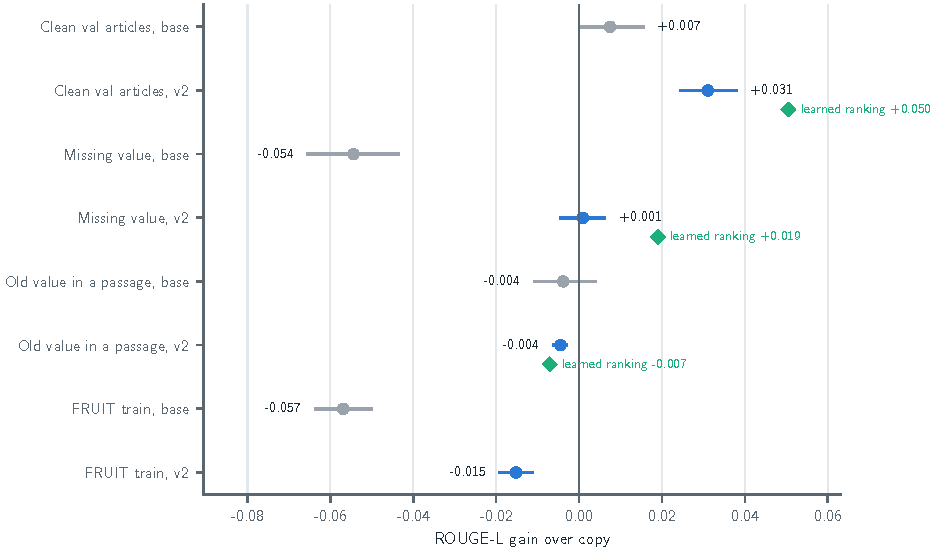
\includegraphics[width=\linewidth]{figures/stress.pdf}
\caption{Sentence ROUGE-L gain over copy on the clean val articles and the stress sets, with 95\% article bootstrap intervals. The diamonds are the learned ranking under cross-validation over the val articles.}
\label{fig:stress}
\end{figure}

\subsection{Cascades and Rounds}

\Cref{fig:loops} shows the loops on the 220 linked test articles. Every detector raises cascade ROUGE-L over the single round, and the consequence head raises it most, from 0.210 to 0.296. The consequence head flags 79\% of the cascade sentences when run once on the gold rewrites of the direct edits, against 72\% for edited as evidence, 29\% for string matching and 14\% for staleness delta. The extra rounds also change sentences that should stay as they are, so \keep{} verbatim falls from 0.929 to 0.898. Gold sentence labels raise UpdateROUGE-L by 0.044 over predicted labels. On the loop sample of 300 test articles, the consequence loop scores 0.014 UpdateROUGE-L above the single round, with an interval of $[0.000, 0.030]$.

\begin{figure}[H]
\centering
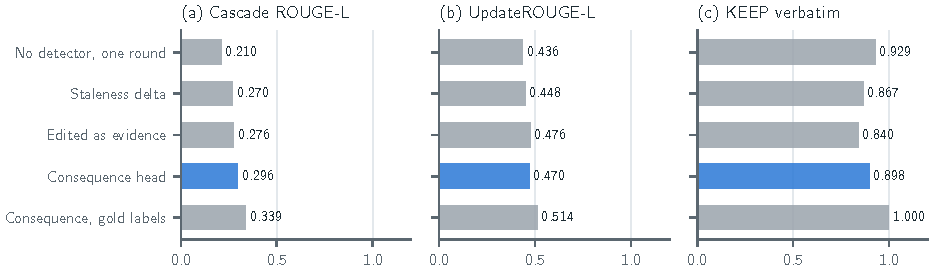
\includegraphics[width=\linewidth]{figures/loops.pdf}
\caption{Loops on the 220 linked test articles. The consequence head is the detector of the current method.}
\label{fig:loops}
\end{figure}

\subsection{Editor Baseline}

The editor reads the outdated article and the evidence and writes the updated article. All of its parameters were trained on the 12,180 train articles. On the 1,670 test sentences it scores 0.973 ROUGE-L, a gain of 0.099 over copy and 0.045 $[0.039, 0.051]$ over \run{fix-rerank}. It corrects 89\% of the new values against 50\% for \run{fix-rerank}, and on the loop sample it reaches UpdateROUGE-L 0.911 against 0.490 for the consequence loop. \Cref{tab:cost} gives the cost. The editor is trained on the train split of the same generator, so it learns the generator's two guarantees from 12,180 examples, and it has not been run on the stress sets.

\begin{table}[H]
\caption{Cost on one A100. Total cost is training plus inference on the 1,602 test articles. The learned ranking adds no GPU time.}
\label{tab:cost}
\centering
\footnotesize
\begin{tabular}{lcc}
\toprule
 & DiffusEdit (\run{fix-rerank}) & T5 editor \\
\midrule
Trained parameters & 12.9M (heads only) & about 780M \\
Training GPU time & about 12 min & 64 min \\
Inference per article & 9.1 s & 0.35 s \\
Total GPU time & about 255 min & about 73 min \\
\bottomrule
\end{tabular}
\end{table}

\section{Limitations}
\label{sec:limits}

The gain of the v2 setting depends on the two guarantees of the generator. It is zero when half of the new values are missing from the evidence and negative when an old value occurs in a passage. The learned ranking keeps a gain on the missing-value set and cannot help on the old-value set, where the veto empties the pool.

The repair rules were designed after the first test run failed gate 1, so the test set had been seen once before the setting was chosen. The setting itself was chosen on val articles that were not used to design the rules, and the learned ranking was fit on those articles and applied to test once.

The stress sets were built after the v2 setting was chosen, on the val articles that chose it. A method designed from the stress results would need a different kind of broken evidence for its final check.

Every repair and loop result comes from one staleness head trained with seed 42. The intervals cover the sampling of articles and not the variation across training seeds.

The editor is fine-tuned on the full train split, while the DiffusEdit infiller is frozen and only its heads are trained. The two are compared on the same test sentences, but they differ in the amount of supervised update text they are trained on.

The ablations run on 300 of the 901 supported test articles, and the loop sample on 300 of 1,602 articles, so their intervals are wider than those of the full test runs.

\bibliographystyle{plainnat}
\bibliography{../paper/paper}

\end{document}
